\section{Детали реализации}

В рамках данной работы было принято решения реализовать требуемые программы на языке \texttt{Java}. Для реализации третьего варианта 
решения задачи было решено использовать парадигму \texttt{MPI}, поскольку существует его расширения для языка программирования 
\texttt{Java} --- \texttt{MPJ Express Project} \footnote{http://mpj-express.org/index.html}. Данная реализация использует нативную
реализацию \texttt{MPI} через \texttt{Java Native Interface} (\texttt{JNI}).

Разработанный в рамках данной работы проект может быть разделен на следующие части:
\begin{itemize}
    \item Классы, описывающие геометрические фигуры и взаимоотношения меджу ними.
    \item Классы, реализующие непосредственно задачу оценки фигуры методом Монте-Карло.
    \item Классы, предназначенные для запуска экспериментов и сбора статистики.
    \item Тестовые классы.
\end{itemize}

Ниже на рисунках \ref{fig:geometry-class-diagram} -- \ref{fig:geometry-performance-diagram} представлены диаграммы классов основных 
частей проекта. 
\begin{figure}[H]
    \centering
    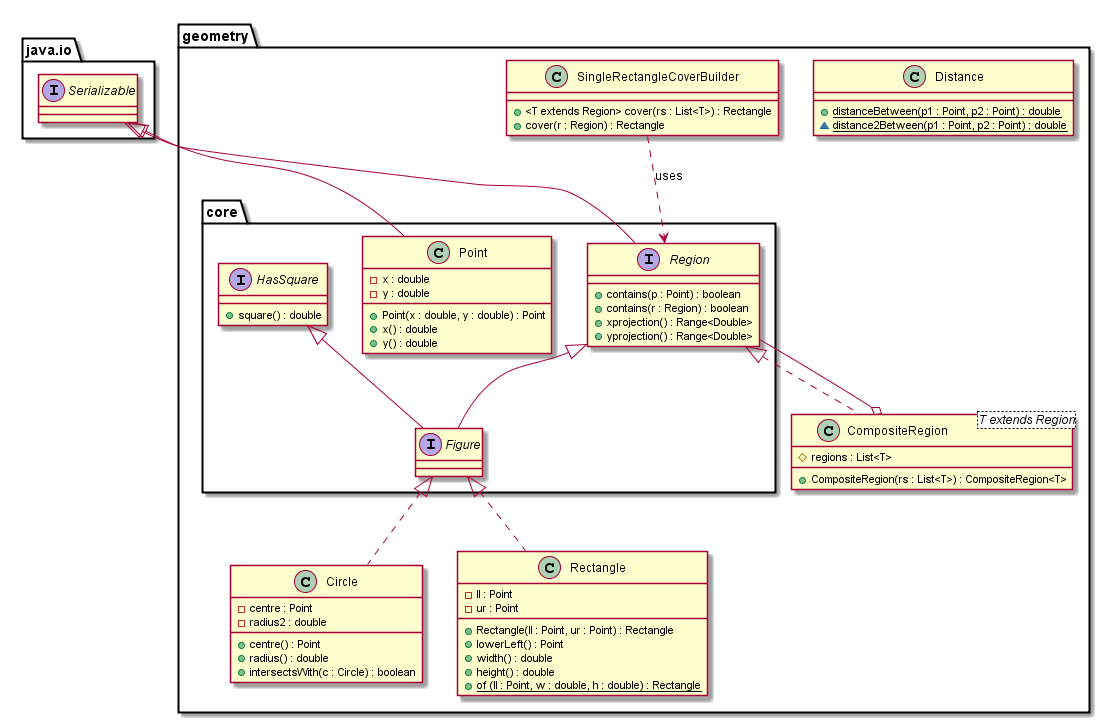
\includegraphics[width=18cm]{resources/diagrams/01_geometry.png}
    \caption{Диаграмма класов для пакета geometry}
    \label{fig:geometry-class-diagram}
\end{figure}
\\ \hfill \\ \hfill
\begin{figure}[H]
    \centering
    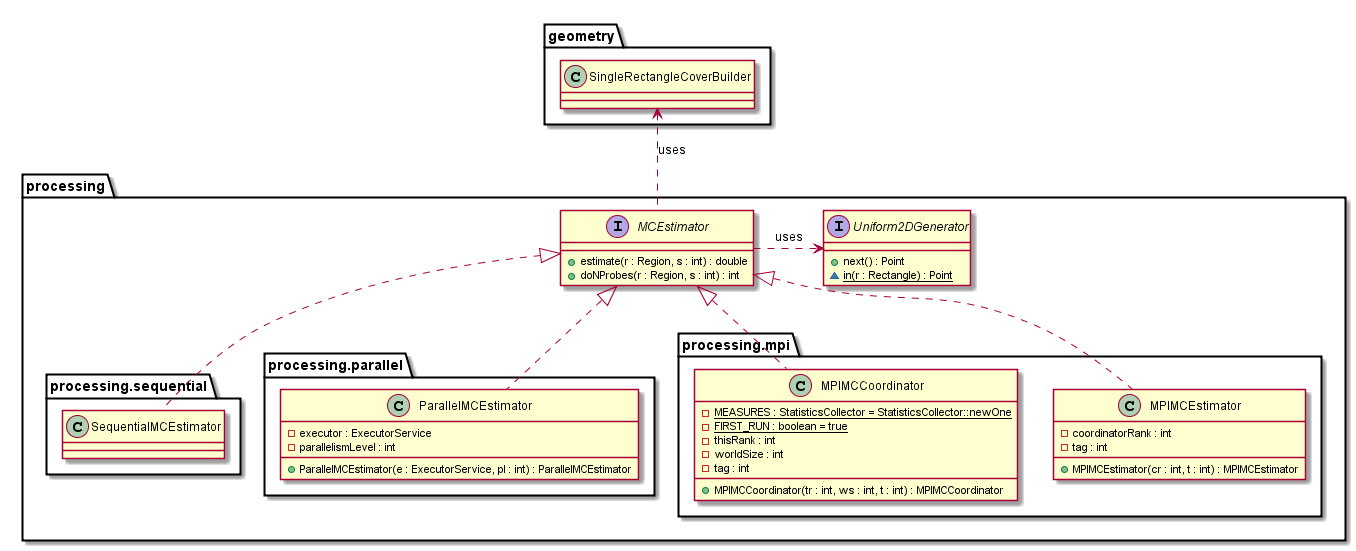
\includegraphics[width=23cm, angle=90]{resources/diagrams/02_processing.png}
    \caption{Диаграмма класов для пакета processing}
    \label{fig:geometry-processing-diagram}
\end{figure}

\begin{figure}[H]
    \centering
    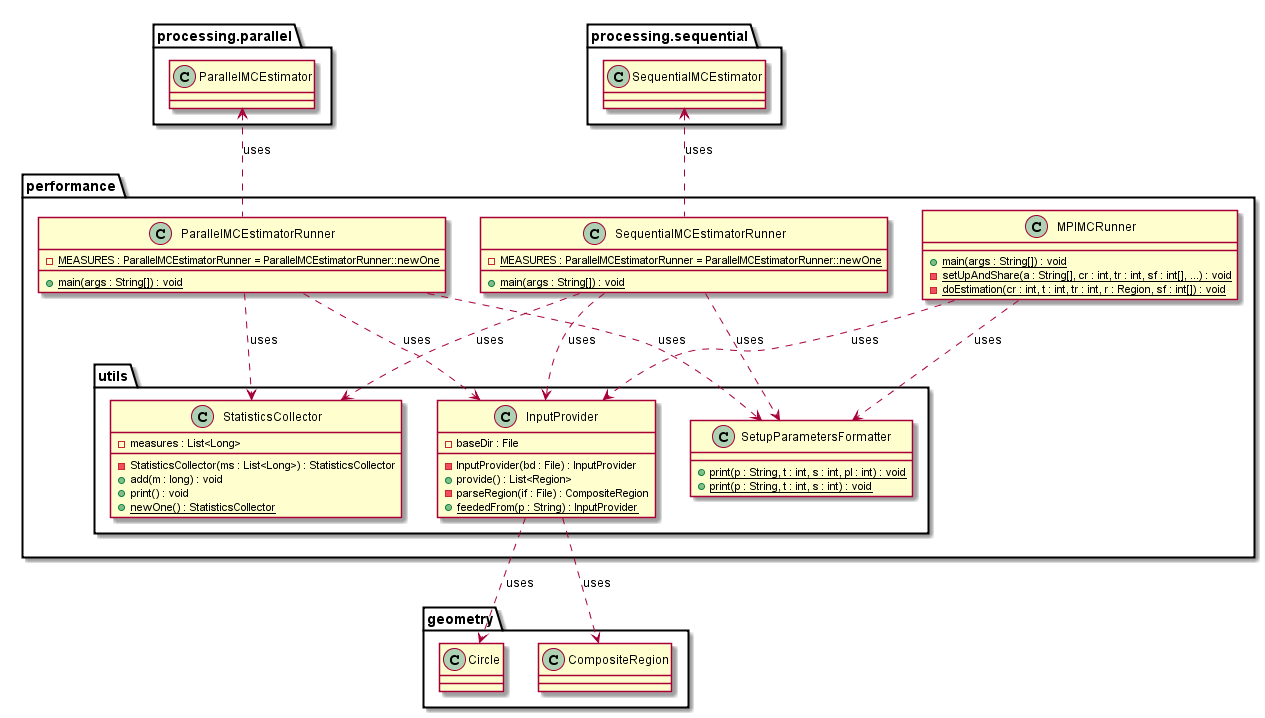
\includegraphics[width=23cm, angle=90]{resources/diagrams/03_performance.png}
    \caption{Диаграмма класов для пакета performance}
    \label{fig:geometry-performance-diagram}
\end{figure}

Ниже в листинге \ref{lst:mc-estimator-src} приведен код класса \texttt{MCEstimator}, реализующего основную функциональность приложения. 
Остальные классы лишь расширяют его (как показано на рисунке \ref{fig:geometry-processing-diagram}), используя функцию 
\texttt{doNProbes} для компонования результатов в случае нескольких потоков.

\begin{listing}[H]
    \inputminted{java}{resources/src/01_MCEstimator}
    \caption{Исзодный код класса MCEstimator}
    \label{lst:mc-estimator-src}
\end{listing}